%%=============================================================================
%% Methodologie
%%=============================================================================

\chapter{\IfLanguageName{dutch}{Methodologie}{Methodology}}%
\label{ch:methodologie}

%% TODO: In dit hoofstuk geef je een korte toelichting over hoe je te werk bent
%% gegaan. Verdeel je onderzoek in grote fasen, en licht in elke fase toe wat
%% de doelstelling was, welke deliverables daar uit gekomen zijn, en welke
%% onderzoeksmethoden je daarbij toegepast hebt. Verantwoord waarom je
%% op deze manier te werk gegaan bent.
%% 
%% Voorbeelden van zulke fasen zijn: literatuurstudie, opstellen van een
%% requirements-analyse, opstellen long-list (bij vergelijkende studie),
%% selectie van geschikte tools (bij vergelijkende studie, "short-list"),
%% opzetten testopstelling/PoC, uitvoeren testen en verzamelen
%% van resultaten, analyse van resultaten, ...
%%
%% !!!!! LET OP !!!!!
%%
%% Het is uitdrukkelijk NIET de bedoeling dat je het grootste deel van de corpus
%% van je bachelorproef in dit hoofstuk verwerkt! Dit hoofdstuk is eerder een
%% kort overzicht van je plan van aanpak.
%%
%% Maak voor elke fase (behalve het literatuuronderzoek) een NIEUW HOOFDSTUK aan
%% en geef het een gepaste titel.
Het onderzoek start met het opstellen van een duidelijke requirementsanalyse. Aan de belanghebbenden van IntelliProve wordt nagevraagd aan welke criteria het model moet voldoen. Deze requirements zijn van belang om de deelvragen voor het onderzoek op te stellen. Deze deelvragen kunnen teruggevonden worden in {~\ref{ch:inleiding}}. \\
\\
Na het definiëren van de requirements kan een uitgebreide literatuurstudie {~\ref{ch:standvanzaken}} worden uitgevoerd. Hierin wordt allerhande informatie verzameld over technieken en modellen. Na het uitvoeren van de literatuurstudie wordt duidelijk beeld gevormd van welke modellen er bestaan en verwerkt kunnen worden in de Proof of Concept. Er wordt ook een flowchart opgesteld van de pipeline. Hieruit kunnen duidelijk alle stappen gehaald worden om de Proof of Concept stapsgewijs te doen verlopen. Deze flowchart kan gevonden worden op figuur {~\ref{fig:pipeline}}\\
\\ 
Uit de informatie en kennis van de literatuurstudie kan het onderzoek worden uitgevoerd als Proof of Concept {~\ref{ch:proofofconcept}. Alle verschillende modellen en technieken kunnen uitgetest worden en geëvalueerd op de dataset.  Het resultaat van de Proof of Concept is een pipeline die op basis van een gezichtsfoto het geslacht en de leeftijd van een persoon gaat voorspellen. \\
\\
Alle resultaten van het onderzoek en eventueel verder onderzoek worden besproken in de Conclusie {~\ref{ch:conclusie}}.

\section{Requirements} \label{sec:meth-requirements} 
\begin{itemize}
    \item De pipeline moet leeftijd en geslacht voorspellen op basis van een frontale gezichtsfoto. Er kan gewerkt worden met 1 machine learning model die beide voorspelt of 2 verschillende modellen die gecombineerd worden tot 1 voorspelde waarde. 
    \item De leeftijd wordt in ranges voorspeld, het gaat dus niet om een exact getal. 
    \item Het geslacht wordt voorspeld op basis van het biologische geslacht, man of vrouw.
    \item De trainings- en test dataset moeten online beschikbaar gesteld zijn. Er is geen interne dataset ter beschikking (omwille van privacy-wetgeving).
    \item De pipeline bestaat uit preprocessing van de afbeelding en het voorspellen van leeftijd en geslacht.
    \item Er is geen opgegeven streefdoel voor de accuraatheid van het model. Dit moet zo hoog mogelijk liggen, maar de conclusies die hieruit getrokken kunnen worden zijn van het grootste belang. Andere modellen kunnen voorgesteld worden, de score kan verklaard worden en toekomstig onderzoek kan aangeboden worden. 
\end{itemize}
\begin{figure}
    \centering
    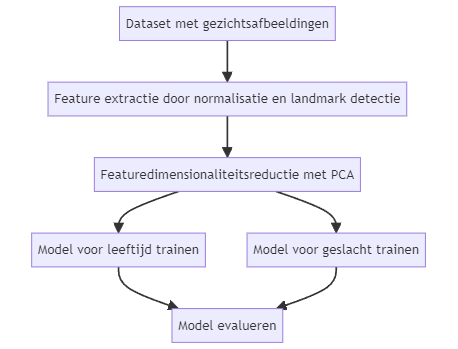
\includegraphics{graphics/pipeline.PNG}
    \caption[Stappen in de pipeline voor Proof of Concept]{\label{fig:pipeline} Stappen in de pipeline voor Proof of Concept}
\end{figure}
 